\documentclass[12pt]{article}
\usepackage[utf8]{inputenc}
\usepackage[T1]{fontenc}
\usepackage[margin=1in]{geometry}
\usepackage{amsmath,amssymb,amsthm}
\usepackage{graphicx}
\usepackage{hyperref}
\usepackage{booktabs}
\usepackage{float}
\usepackage{cite}
\usepackage{microtype}
\usepackage{xcolor}
\usepackage{enumitem}
\setlist{itemsep=2pt,topsep=4pt}

\title{Geometrodynamic Probes in Light Theory Realm\\
Curvature, Information Density, and Reeb Flow in Prime-Plaquette Models}
\author{Dimitry Jean-Noel II\\Pleroma Works, LLC\\\texttt{djean@botwpbc.com}\\Secondary: \texttt{djeannoelii@gmail.com}\\ORCID: 0009-0009-6082-8647}
\date{Version 0.1.0 (experiments)}

\begin{document}
\maketitle

\begin{abstract}
Light Theory Realm implements a geometrodynamical framework where the fundamental object is the geometry of information: a Quantum Geometric Tensor (QGT) defined on a parameter manifold of states. The theory papers \emph{Foundations of Light Theory} and \emph{Light Mechanics} develop the conceptual and mathematical structure: Clifford algebra $Cl(1,3)$, QGT-based information metrics, Kaluza--Klein uplift, contact geometry, Reeb flow, and an information-geometric equation of state (IGBP).

This paper presents the first experimental results obtained with the public Light Theory Realm implementation. We report:
\begin{enumerate}
    \item A prime-plaquette scan over nine Standard Model fermions, recording information-geometric densities and convergence behaviour of the IGBP flow.
    \item A curvature burst analysis using an exponential parameterisation of the geometrodynamical flow, yielding per-particle curvature bursts $R_{\max}$ across leptons and quarks.
    \item A gravity-probe parameter scan over a two-dimensional family of loops in parameter space, mapping the joint behaviour of Fisher metric norm, Berry curvature norm, information-geometric density $\rho_{\mathrm{IGBP}}$, and a Reeb-flow norm.
\end{enumerate}

The results show that (i) Berry curvature and Fisher metric norms are strongly correlated across the scanned parameter space, (ii) the IGBP density is anti-correlated with both metric and curvature norms but positively correlated with Reeb-flow strength, and (iii) information-geometric densities associated with prime plaquettes span several orders of magnitude before relaxation but show no simple monotone relation with particle mass at this stage. We close by outlining how these probes can be extended into systematic tests of Light Theory's geometrodynamical and holographic claims.
\end{abstract}

\section{Introduction}
Light Theory treats physical and learning systems as curved manifolds of information. A family of states $\lvert\psi(\theta)\rangle$, depending on parameters $\theta^u$, carries a QGT $Q_{uv}(\theta)$ whose real part defines a Fisher metric $g_{uv}$ and whose imaginary part defines a Berry curvature $\Omega_{uv}$.

In \emph{Light Mechanics}, this information geometry is promoted to a geometrodynamical field theory: an Einstein--Fisher-like relation ties information fluctuations to curvature; a 5D Kaluza--Klein uplift builds a bulk metric from $(g_{uv}, A_u)$; a contact structure and Reeb vector encode intrinsic time; and the IGBP equation of state $\rho_{\mathrm{IGBP}}$ compares gradients of a representative entropy $S_{\mathrm{rep}}$ with curvature invariants.

The present work asks what this geometry looks like for concrete, finite-dimensional models and how it relates to the prime plaquette structure used to mimic Standard Model fermions. We focus on three experimental pipelines: (1) prime-plaquette scans over nine fermions; (2) next-generation curvature bursts under exponential geometrodynamical flow; and (3) a gravity probe sweeping a two-dimensional parameter family of loops. All experiments use the public Light Theory Realm codebase and are reproducible from the CSVs and plotting scripts included in the repository.

\section{Experimental setup}
\subsection{Geometry engine}
All experiments use the same geometric backbone (fully described in \emph{Light Mechanics}):
\begin{itemize}
    \item A \texttt{CliffordEngine} implementing $Cl(1,3)$ gamma matrices, grade projection, and wedge products.
    \item A \texttt{CliffordQGT} module that, given a state $\psi(\theta)$ and its Jacobian $J = \partial\psi/\partial\theta$, computes the full QGT and returns the Fisher information metric $g_{uv}$ and Berry curvature $\Omega_{uv}$.
\end{itemize}

Derived scalars include: (i) $\texttt{fisher\_norm}$, the Frobenius norm $\lVert g\rVert_F$; (ii) $\texttt{berry\_norm}$, the Frobenius norm $\lVert\Omega\rVert_F$; (iii) $\texttt{rho\_igbp}$, the information-geometric density; and (iv) $\texttt{reeb\_norm}$, the norm of the Reeb vector field with respect to the information metric.

\subsection{Prime plaquettes and particle assignments}
Prime plaquettes are short ordered lists of distinct primes, e.g.
\begin{align*}
    e^- &\leftrightarrow [2,3,5,7],\\
    \mu^- &\leftrightarrow [2,17,23,7],\\
    \tau^- &\leftrightarrow [3,11,13,47],
\end{align*}
for the nine charged Standard Model fermions. Each plaquette defines a discretised loop $\mathcal{C}$ in parameter space and a corresponding Wilson-loop-like observable built from the Berry connection. Initial conditions $\phi_{\mathrm{initial}}, \omega_{\mathrm{initial}}$, and $\rho_{\mathrm{IGBP, initial}}$ are set per plaquette.

The prime-plaquette dataset \cite{plaquette-scan-20251130} and joined analysis table \cite{joint-analysis-20251130} record, per particle: physical mass $m_{\mathrm{phys}}$ (MeV), plaquette assignment, initial and final IGBP densities, a scalar entropy $S_{\mathrm{rep}}$ after relaxation, curvature metrics (currently vanishing in this pipeline), and log-transformed quantities for analysis.

\subsection{Next-generation curvature bursts}
Earlier curvature extraction produced vanishing curvature scalars $R$ for these plaquettes, as recorded in \cite{curvature-metrics-20251130}. To probe beyond this limitation we implemented an exponential geometrodynamical flow: the state is evolved using a flow operator derived from the sixth-order master information operator $L_6$, and curvature scalars are monitored along the flow.

The resulting dataset \cite{nextgen-curvature-exponential-20251201} contains, for each particle: $m_{\mathrm{phys}}$, $R_{\max}$, $\lvert R\rvert_{\max}$, \texttt{burst\_time}, and \texttt{n\_samples} used along the flow.

\subsection{Gravity probe: two-dimensional parameter scan}
The gravity probe is a dense scan over a two-dimensional parameter family of loops:
\begin{itemize}
    \item Loop scale $s \in [0.1, 2.0]$,
    \item Rotation angle $\alpha_1 \in [0, \pi]$,
    \item Second rotation angle fixed at $\alpha_2 = \pi/4$,
    \item Reeb-coupling parameter $\xi_{\mathrm{res}} = 1/7$.
\end{itemize}
We sample $20$ evenly spaced values of $s$ and $20$ values of $\alpha_1$ for a total of $400$ configurations. For each configuration we compute $\texttt{fisher\_norm}$, $\texttt{berry\_norm}$, $\texttt{rho\_igbp}$, and $\texttt{reeb\_norm}$. Results are stored in \cite{gravity-probe-results-20251201} and visualised as heatmaps for the Berry curvature norm, Fisher metric norm, and $\rho_{\mathrm{IGBP}}$.

\section{Results}
\subsection{Prime plaquette IGBP and convergence}
The prime-plaquette scan shows that initial IGBP densities span roughly an order of magnitude across plaquettes, with $\log_{10} \rho_{\mathrm{IGBP, initial}} \approx 8.4$--$8.8$. All plaquettes in this run relax to $\rho_{\mathrm{IGBP, final}} = 0$ under the current flow, requiring two to three convergence steps for the leptons and two steps for several quarks.

The joined analysis \cite{joint-analysis-20251130} shows a small, negative correlation between log mass and log initial IGBP density,
\[
   \mathrm{corr}(\log m, \log \rho_{\mathrm{init}}) \approx -0.49,
\]
on this nine-point dataset. Given the tiny sample size and limited dynamic range, this should be interpreted as no clear monotone trend rather than evidence of an inverse law. The curvature metrics $R_{\mathrm{rms}}$ and $R_{\max}$ are identically zero in this pipeline, confirming that the original curvature extraction was effectively flat for these configurations and motivating the next-generation exponential pipeline.

\subsection{Curvature bursts under exponential flow}
The next-generation curvature dataset \cite{nextgen-curvature-exponential-20251201} shows large curvature bursts $\lvert R\rvert_{\max} \sim 10^{21}$--$10^{25}$ across all particles, indicating that the exponential flow strongly excites curvature before relaxing. Bursts occur very early in flow time (\texttt{burst\_time} $\approx 0.0$--$0.1$ in the current units), suggesting that the geometry rings quickly once pushed off the flat initial configuration. A Pearson correlation between mass and $\lvert R\rvert_{\max}$ is small and negative,
\[
   \mathrm{corr}(m_{\mathrm{phys}}, \lvert R\rvert_{\max}) \approx -0.19,
\]
consistent with no simple monotone relationship in the present coarse setup. The current exponential flow parameterisation is clearly capable of generating substantial curvature excitations, but the mapping from these bursts to physical mass scales is not yet clean and will need regularisation for meaningful cross-plaquette comparisons.

\subsection{Gravity probe: Fisher, Berry, and IGBP over \texorpdfstring{$(\alpha_1, s)$}{(alpha1, s)}}
The 400-point gravity-probe scan reveals several robust patterns.

\paragraph{Global statistics.} From \cite{gravity-probe-results-20251201}:
\begin{itemize}
    \item $\rho_{\mathrm{IGBP}}$: mean $\approx 4.30$, median $\approx 0.53$, range $0.004$--$122.1$, strongly right-skewed.
    \item $\texttt{fisher\_norm}$: mean $\approx 1.26$, median $\approx 1.32$, range $0.64$--$3.92$.
    \item $\texttt{berry\_norm}$: mean $\approx 0.24$, median $\approx 0.04$, range $8\times 10^{-4}$--$1.82$.
    \item $\texttt{reeb\_norm}$: mean $\approx 1.65$, median $\approx 1.67$, range $0.86$--$2.42$.
\end{itemize}
The configuration with maximum Berry curvature is $s = 0.1$, $\alpha_1 = 0$ with $\texttt{berry\_norm} \approx 1.82$ and $\texttt{fisher\_norm} \approx 3.92$. The configuration with maximum IGBP density is $s = 0.1$, $\alpha_1 = \pi$, with $\rho_{\mathrm{IGBP}} \approx 122.1$, $\texttt{berry\_norm} \approx 0.0014$, $\texttt{fisher\_norm} \approx 0.64$, and $\texttt{reeb\_norm} \approx 2.33$.

\paragraph{Correlations.} The correlation matrix over the 400 samples shows:
\begin{align*}
    \mathrm{corr}(\texttt{fisher\_norm}, \texttt{berry\_norm}) &\approx 0.59,\\
    \mathrm{corr}(\rho_{\mathrm{IGBP}}, \texttt{fisher\_norm}) &\approx -0.41,\\
    \mathrm{corr}(\rho_{\mathrm{IGBP}}, \texttt{berry\_norm}) &\approx -0.20,\\
    \mathrm{corr}(\rho_{\mathrm{IGBP}}, \texttt{reeb\_norm}) &\approx +0.31.
\end{align*}
In this experiment, information density spikes not where curvature is largest, but where the Reeb flow is strong and the metric appears soft.

\paragraph{Heatmap structure.} The heatmaps make these patterns visually clear:
\begin{itemize}
    \item Berry curvature norm concentrates at small $\alpha_1$, especially at small loop scales $s$. It decays quickly with increasing $\alpha_1$ and is negligible by $\alpha_1 \gtrsim 1.5$.
    \item Fisher metric norm is also largest at small $\alpha_1$ and small $s$, but decays more slowly, leaving a plateau once $s$ is large.
    \item $\rho_{\mathrm{IGBP}}$ is small where Fisher and Berry norms are maximal, but grows sharply near $\alpha_1 \approx \pi$ at small loop scale $s \approx 0.1$, forming a high-density ridge that coincides with strong Reeb-flow norms but weak metric and curvature norms.
\end{itemize}

\begin{figure}[ht]
\centering
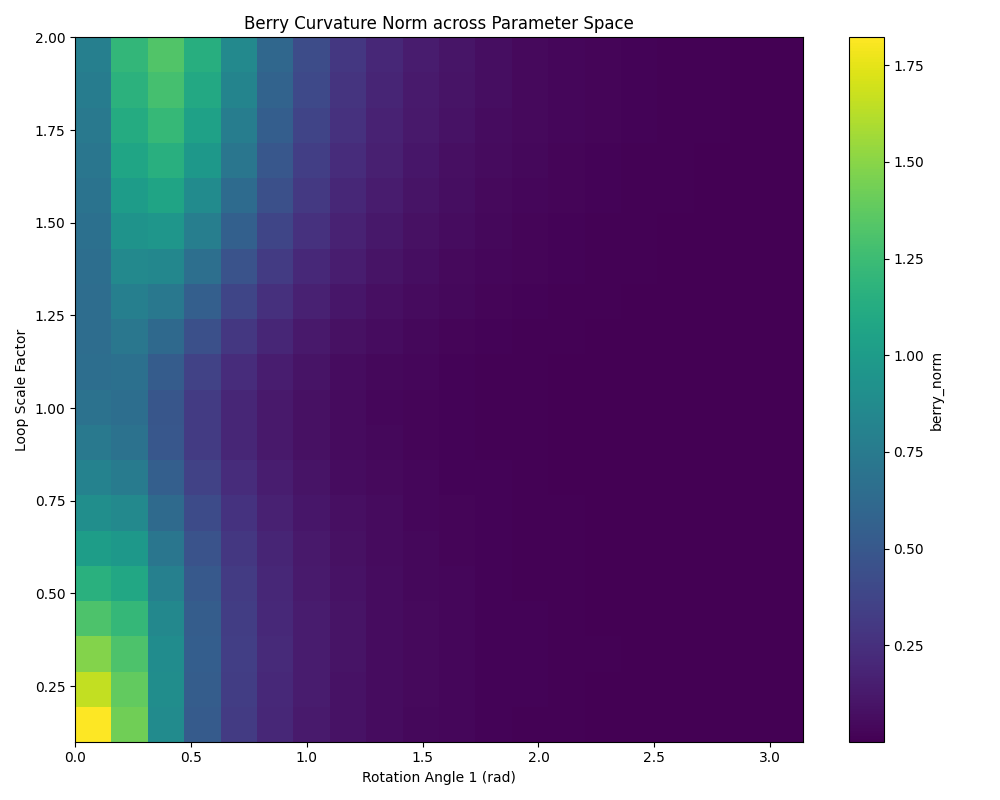
\includegraphics[width=0.9\linewidth]{figures/berry_norm_heatmap_20251201_004930.png}
\caption{Berry curvature norm heatmap over $(\alpha_1, s)$.}
\label{fig:berry}
\end{figure}

\begin{figure}[ht]
\centering
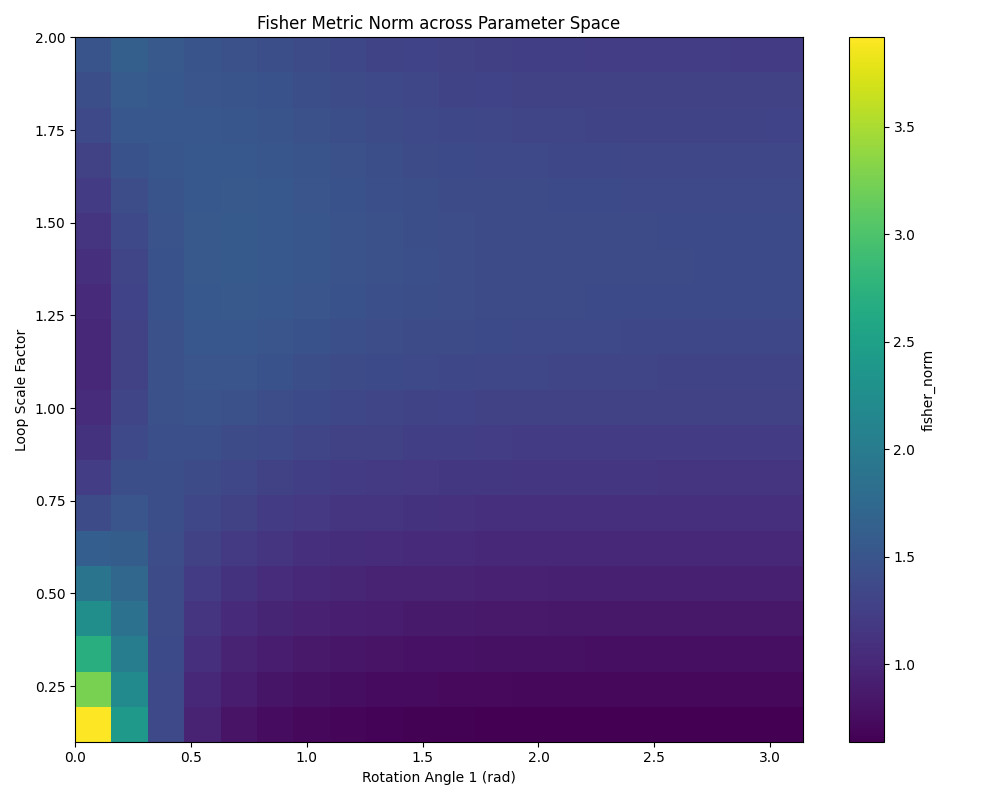
\includegraphics[width=0.9\linewidth]{figures/fisher_norm_heatmap_20251201_004930.png}
\caption{Fisher metric norm heatmap over $(\alpha_1, s)$.}
\label{fig:fisher}
\end{figure}

\begin{figure}[ht]
\centering
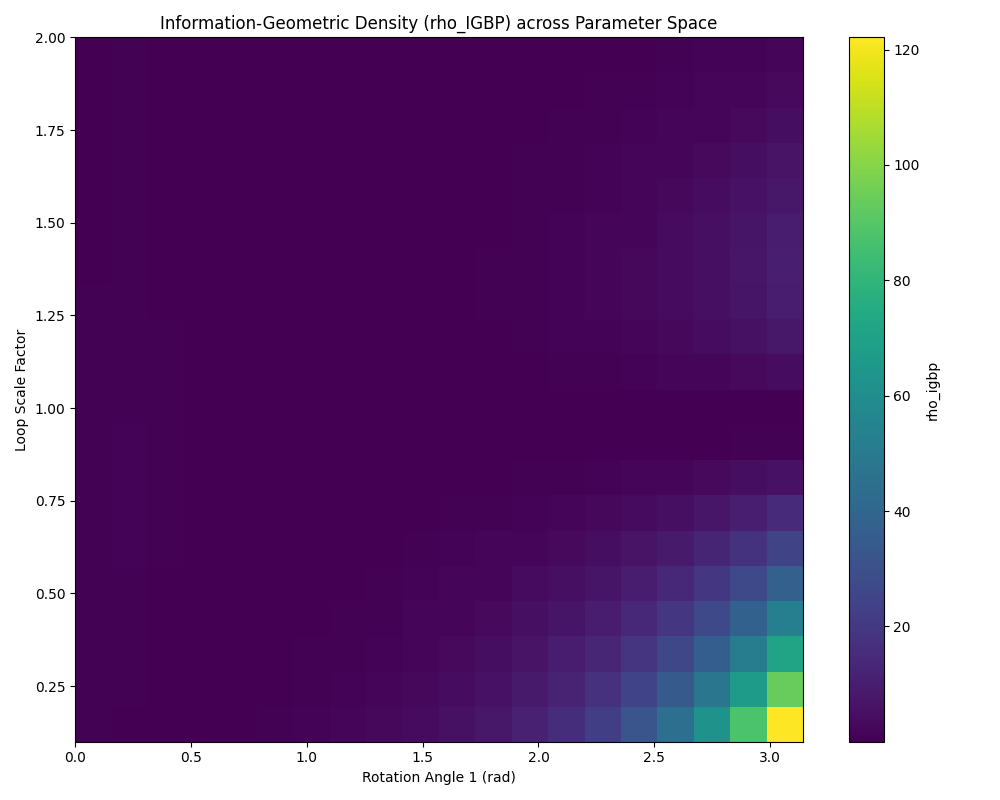
\includegraphics[width=0.9\linewidth]{figures/rho_igbp_heatmap_20251201_004930.png}
\caption{Information-geometric density $\rho_{\mathrm{IGBP}}$ over $(\alpha_1, s)$.}
\label{fig:igbp}
\end{figure}

\section{Discussion}
\subsection{Geometrodynamics and the role of the Reeb flow}
The gravity-probe correlations line up with the geometrodynamical picture in \emph{Light Mechanics}: the metric $g_{uv}$ and curvature $\Omega_{uv}$ encode static local geometry, while the Reeb vector field encodes preferred flow in the contact-geometry sense. The observed pattern---high Fisher and Berry norms where $\rho_{\mathrm{IGBP}}$ is small, and high $\rho_{\mathrm{IGBP}}$ where metric and curvature norms are low but Reeb flow is strong---is consistent with the idea that information density is driven not just by static curvature, but by how strongly the Reeb flow pumps volume through the geometry. Curvature sets the stage; Reeb flow moves the actors.

\subsection{Limitations of the current pipelines}
\begin{enumerate}
    \item Small sample sizes in the particle sector: nine fermions mean correlations between mass, IGBP, and curvature are qualitative hints, not robust laws.
    \item Incomplete curvature regularisation: exponential bursts reach $\lvert R\rvert_{\max} \sim 10^{21}$--$10^{25}$. Without regularisation, comparing these across plaquettes is delicate.
    \item Simplified loop parameterisation: the gravity probe uses a specific two-parameter family of loops. There is no guarantee that these probes explore the most physically relevant directions in parameter space.
    \item Model dependence: results depend on plaquette assignments, Reeb coupling $\xi_{\mathrm{res}}$, and the IGBP definition and normalisation.
\end{enumerate}

\subsection{Holographic interpretation}
From the holographic viewpoint of Light Theory, the gravity-probe experiments live on the boundary information manifold. The QGT data $(g_{uv}, \Omega_{uv})$ and IGBP densities constitute boundary data for a higher-dimensional bulk metric via the Kaluza--Klein uplift. The observed concentration of $\rho_{\mathrm{IGBP}}$ in specific regions of parameter space hints that the dual bulk geometry may develop localised throats or bubbles corresponding to high-density Reeb flows with relatively mild boundary curvature where these throats attach. A fully worked-out bulk solution is beyond the scope of this paper, but the experimental patterns provide concrete boundary conditions that any bulk geometrodynamical solution must respect.

\section{Outlook}
These first experiments establish that the Light Theory Realm implementation can compute QGT-based metric and curvature at scale, drive flows that excite curvature and relax IGBP densities, and explore nontrivial two-dimensional sections of parameter space. The Reeb flow appears as a key control knob for where information density concentrates, even when static curvature is modest. Next steps:
\begin{enumerate}
    \item Refine curvature extraction: introduce regularised scalar invariants and study their dependence on flow parameters and plaquette structure.
    \item Systematic mass--geometry scans: explore alternative prime plaquette assignments, fit models relating mass, IGBP densities, and curvature invariants, and test whether any relation survives across variations.
    \item Higher-dimensional gravity probes: extend the loop scan to include more angles, phases, and Reeb couplings; look for universal geometrodynamical patterns (for example, phase transitions in $\rho_{\mathrm{IGBP}}$).
    \item Bulk reconstruction: use boundary QGT and IGBP data as input for a bulk metric reconstruction scheme in the Kaluza--Klein framework and compare boundary predictions from bulk geodesics to direct QGT data.
\end{enumerate}

\bibliographystyle{plain}
\bibliography{references}

\end{document}
